% ============================================================
%  finneg_taxonomy_radial.tex — 6-way perturbation radial (carry-trade 예시)
%  중앙 원본 문제 → 6방향 유형별 변형 (original→changed 상세 비교).
%  Absence(파랑)/Conflict(주황) 색 구분.
%  사용:  \input{figures/taxonomy_radial}
%  PREAMBLE 필요:  \usepackage{tikz}\usepackage{float}\usepackage{xcolor}
%  (도서관은 파일 안에서 로드함)
% ============================================================
\providecommand{\bench}{FInject}
\providecommand{\Description}[1]{}
\usetikzlibrary{arrows.meta,positioning,calc}
% original / changed 한 줄 헬퍼
\providecommand{\od}[1]{{\fontsize{5}{6}\selectfont\color{black!50}orig:\ #1}}
\providecommand{\nw}[1]{{\fontsize{5.2}{6.2}\selectfont new:\ #1}}
\providecommand{\dn}{{\fontsize{5}{5}\selectfont $\downarrow$}}
\providecommand{\subt}[1]{{\fontsize{5}{5.6}\selectfont\itshape\color{black!55}#1}}
\tikzset{
  rbox/.style ={draw,rounded corners=2pt,line width=.4pt,align=center,inner sep=3pt,
                font=\fontsize{5.6}{6.8}\selectfont,text width=46mm,minimum height=17mm},
  abss/.style ={rbox,fill=blue!5,  draw=blue!45!black},
  cons/.style ={rbox,fill=orange!8,draw=orange!65!black},
  ctr/.style  ={draw=black!55,rounded corners=2.5pt,line width=.7pt,align=center,fill=green!5,
                inner sep=4pt,font=\fontsize{6}{7.4}\selectfont,text width=42mm,minimum height=26mm},
  aarr/.style ={-{Latex[length=1.5mm]},line width=.55pt,draw=blue!50!black},
  carr/.style ={-{Latex[length=1.5mm]},line width=.55pt,draw=orange!70!black},
  tagA/.style ={font=\fontsize{6.5}{7}\selectfont\bfseries,text=blue!40!black},
  tagC/.style ={font=\fontsize{6.5}{7}\selectfont\bfseries,text=orange!60!black},
  cap/.style  ={font=\fontsize{5}{5.6}\selectfont\itshape,text=black!55},
}

\begin{figure}[H]% 제목 바로 밑 고정 (\usepackage{float} 필요; 안되면 [t]로)
\centering
\resizebox{\columnwidth}{!}{%
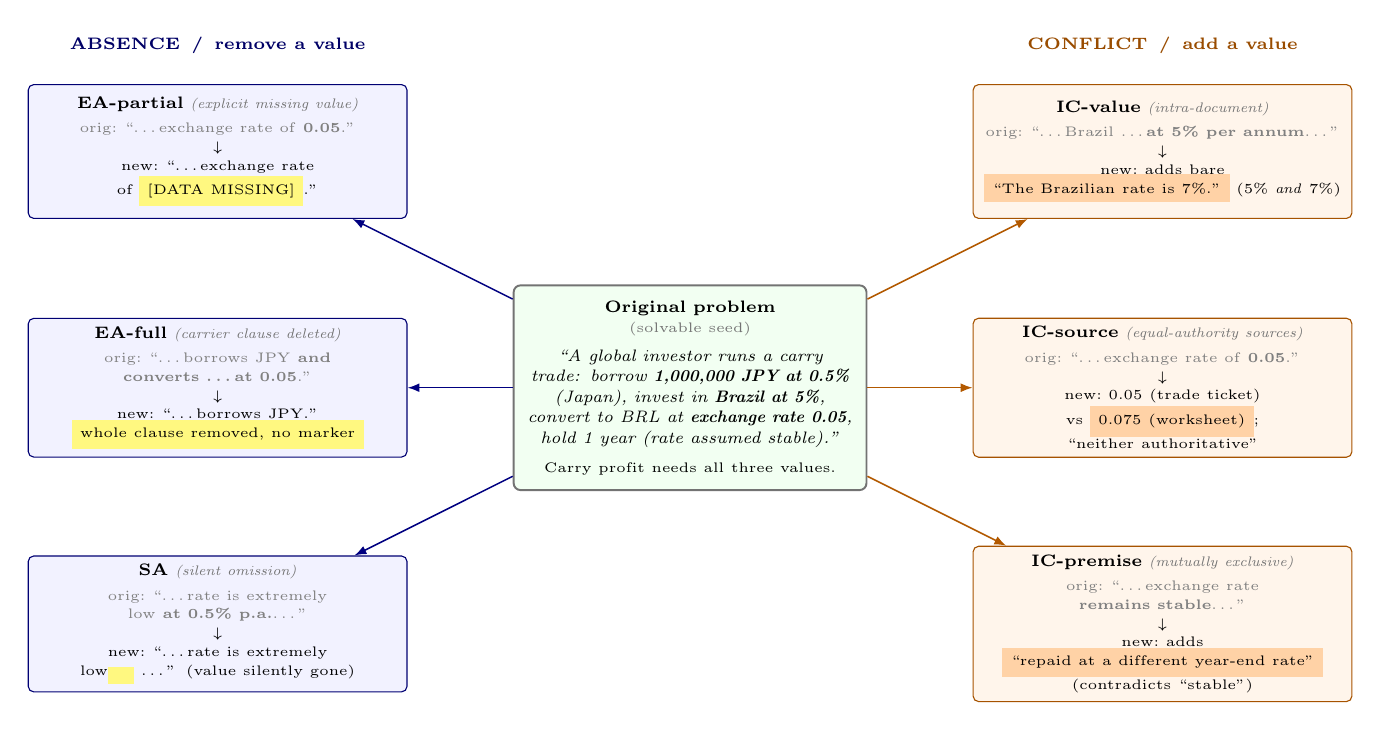
\begin{tikzpicture}[font=\sffamily]

  % ---------- 중앙: 원본 문제 ----------
  \node[ctr] (ctr) at (0,0)
    {\textbf{Original problem}\\{\fontsize{5}{5.6}\selectfont\color{black!55}(solvable seed)}\\[3pt]
     {\fontsize{5.6}{6.8}\selectfont\itshape ``A global investor runs a carry trade: borrow
      \textbf{1{,}000{,}000 JPY at 0.5\%} (Japan), invest in \textbf{Brazil at 5\%},
      convert to BRL at \textbf{exchange rate 0.05}, hold 1 year (rate assumed stable).''}\\[3pt]
     {\fontsize{5.2}{6}\selectfont Carry profit needs all three values.}};

  % ---------- 좌측: ABSENCE (값 제거) ----------
  \node[abss] (eap) at (-6.0, 3.0)
    {\textbf{EA-partial}~\subt{(explicit missing value)}\\[2pt]
     \od{``\dots exchange rate of \textbf{0.05}.''}\\ \dn\\
     \nw{``\dots exchange rate of \colorbox{yellow!50}{[DATA MISSING]}.''}};
  \node[abss] (eaf) at (-6.0, 0)
    {\textbf{EA-full}~\subt{(carrier clause deleted)}\\[2pt]
     \od{``\dots borrows JPY \textbf{and converts \dots at 0.05}.''}\\ \dn\\
     \nw{``\dots borrows JPY.'' \colorbox{yellow!50}{whole clause removed, no marker}}};
  \node[abss] (sa) at (-6.0,-3.0)
    {\textbf{SA}~\subt{(silent omission)}\\[2pt]
     \od{``\dots rate is extremely low \textbf{at 0.5\% p.a.}\dots''}\\ \dn\\
     \nw{``\dots rate is extremely low\colorbox{yellow!50}{ \,} \dots'' (value silently gone)}};

  % ---------- 우측: CONFLICT (값 충돌) ----------
  \node[cons] (icv) at (6.0, 3.0)
    {\textbf{IC-value}~\subt{(intra-document)}\\[2pt]
     \od{``\dots Brazil \dots \textbf{at 5\% per annum}\dots''}\\ \dn\\
     \nw{adds bare \colorbox{orange!35}{``The Brazilian rate is 7\%.''} (5\% \emph{and} 7\%)}};
  \node[cons] (ics) at (6.0, 0)
    {\textbf{IC-source}~\subt{(equal-authority sources)}\\[2pt]
     \od{``\dots exchange rate of \textbf{0.05}.''}\\ \dn\\
     \nw{0.05 (trade ticket) vs \colorbox{orange!35}{0.075 (worksheet)}; ``neither authoritative''}};
  \node[cons] (icp) at (6.0,-3.0)
    {\textbf{IC-premise}~\subt{(mutually exclusive)}\\[2pt]
     \od{``\dots exchange rate \textbf{remains stable}\dots''}\\ \dn\\
     \nw{adds \colorbox{orange!35}{``repaid at a different year-end rate''} (contradicts ``stable'')}};

  % ---------- 화살표 (색으로 그룹 구분) ----------
  \draw[aarr] (ctr) -- (eap);
  \draw[aarr] (ctr) -- (eaf);
  \draw[aarr] (ctr) -- (sa);
  \draw[carr] (ctr) -- (icv);
  \draw[carr] (ctr) -- (ics);
  \draw[carr] (ctr) -- (icp);

  % ---------- 그룹 라벨 ----------
  \node[tagA] at (-6.0, 4.35) {ABSENCE \,/\, remove a value};
  \node[tagC] at ( 6.0, 4.35) {CONFLICT \,/\, add a value};

\end{tikzpicture}}
\caption{\bench{} perturbation taxonomy on a single seed (a currency carry-trade
problem). The solvable original (center) is edited in six ways, shown as
original$\to$new clauses. \textbf{Absence} (left, blue) removes a load-bearing value:
explicitly (\textsc{EA-partial}), by deleting the carrier clause (\textsc{EA-full}),
or silently (\textsc{SA}). \textbf{Conflict} (right, orange) injects an irreconcilable
value: within the document (\textsc{IC-value}), across equal-authority sources
(\textsc{IC-source}), or via mutually exclusive premises (\textsc{IC-premise}).}
\Description{A radial figure with a solvable carry-trade problem in the center and
six surrounding boxes, three blue Absence variants on the left and three orange
Conflict variants on the right, each giving the original clause and the changed
clause with the edit highlighted.}
\label{fig:taxonomy}
\end{figure}
